
\chapter{Improving precision}
% \section{Deriving information from boolean expressions}
%As the analysis is now, we have a crude over-approximation, and in order to improve that, we can harvest more %information from the flow graph.\\\\
%Up until now, we did not care about the conditions for loops or branches. For instance, given the code in figure %\ref{fig:if_flow_example}, we \emph{could} derive information about the state of the variable y, depending on %which branch we take. In essence, if we take the true branch, we know for certain that the value of y, is indeed %the value of x - which is 5 (but that is less interesting in this case). If -- on the other hand -- we take the %false branch, we know for certain that the value of y is \emph{every other value} than those of x.\\\\
%\begin{figure}[h]
%\centering
%\begin{tikzpicture}[->,>=stealth',shorten >=1pt,auto,node distance=2.5cm,
%                    semithick]
%   \tikzstyle{block} = [rectangle, draw, fill=none, 
%    text width=5em, text centered, rounded corners, minimum height=3em]
%    
%  \node[block] (1) {[x:=5]$^1$};
%  \node[block] (2) [below of=2]  {if [x=y]$^2$};
%  \node[block] (3) [below left of=2]  {[y:=x+2]$^3$};
%  \node[block] (4) [below right of=2]  {[y:=x-2]$^4$};
%  \node[block] (5) [below right of=3]  {[write~y]$^5$};
%
%  
%  \path (1) edge  node {} (2)
%        (2) edge  node {} (3)
%            edge  node {} (4)
%        (3) edge  node {} (5)
%        (4) edge  node {} (5);
%
%\end{tikzpicture}
% \caption{}
% \label{fig:if_flow_example}
%\end{figure} In order to raise this to a more general level, we follow the suggestion from \cite{02242_slides} %and map two transfer functions to the statements corresponding to if and while, rather than one.

%TODO More stuff about this, and link it together with the paragraph above. (and stuff).

%We will then use the functions defined table \ref{table:expression_mapping}. The basic idea, starting from $a_1 = %a_2$, is that if we have two sets with definitions; then we can only enter the true branch if $\mathcal{A_S}[\![a_1]\!]$ and $\mathcal{A_S}[\![a_2]\!]$ have the same values. Thus, the only viable definitions that are allow to be passed along to the true branch, are the definitions that are both in $\mathcal{A_S}[\![a_1]\!]$ and $\mathcal{A_S}[\![a_2]\!]$. Hence, the intersection.\\\\
%The $a_1 \neq a_2$ then becomes the complimentary set to the one from $a_1 = a_2$, the $a_1 < a_2$ %TODO complete this, and verify the table.

%\subsection{Handling arithmetic expressions}
%\begin{table}
%\centering
%\begin{tabular}{|r|l|}
%\hline
%Expression & Definition \\
%\hline
%$ a_1 = a_ 2$     & $ \mathcal{A_S}[\![a_1]\!] \bigcap \mathcal{A_S}[\![a_2]\!] $ \\
%$ a_1 \neq a_ 2$  &  $ \left(\mathcal{A_S}[\![a_1]\!] \bigcap \mathcal{A_S}[\![a_2]\!]\right) \setminus \left(\mathcal{A_S}[\![a_1]\!]) \bigcup (B_{=} \setminus \mathcal{A_S}[\![a_2]\!]\right) $ \\
%$ a_1 < a_ 2$     & $ \mathcal{A_S}[\![a_1]\!] \bigcup \left(\mathcal{A_S}[\![a_1]\!] \setminus \mathcal{A_S}[\![a_2]\!]\right) $ \\
%$ a_1 > a_ 2$     & $ \mathcal{A_S}[\![a_2]\!] \bigcup \left(\mathcal{A_S}[\![a_2]\!] \setminus \mathcal{A_S}[\![a_1]\!]\right) $ \\
%$ a_1 \leq a_ 2$  & $ \mathcal{A_S}[\![a_1]\!] \bigcup \left(\mathcal{A_S}[\![a_1]\!] \setminus \mathcal{A_S}[\![a_2]\!]\right) \bigcup \left(\mathcal{A_S}[\![a_1]\!] \bigcap \mathcal{A_S}[\![a_2]\!]\right) $ \\
%$ a_1 \geq a_2$   & $ \mathcal{A_S}[\![a_2]\!] \bigcup \left(\mathcal{A_S}[\![a_2]\!] \setminus \mathcal{A_S}[\![a_1]\!]\right) \bigcup  \left(\mathcal{A_S}[\![a_1]\!] \bigcap \mathcal{A_S}[\![a_2]\!]\right)$ \\
%\hline
%\end{tabular}
%\caption{Expression mapping}
%\label{table:expression_mapping}
%\end{table}


\section{Overflow detection optimizations}
The interval analysis we are performing for while-loops assumes that the body is executed once, hence the result of the interval analysis performed in the body is an under approximation, since there is potential for that the body will be executed multiple times.\\\\
However,	 the obtained results are indeed a part of the precise result, but on the other hand we might omit some of the results for interval analysis which might result an imprecise result for detection of buffer overflow.
If we could guarantee a number of iterations that the body would execute, we could do an optimization such as we could get a more exact result for the interval analysis by performing the analysis as the same number of iterations for the statements in the body.\\\\
A reason for why we can not calculate the number of iterations for how many times the loop is executed is because it might be depended on the body, and it would require advanced analysis to calculate this number.
Another approach for how the interval analysis could be performed for while-loop is to a assume that the body will run infinity often, and then extend out \mathcal{F} space with additional functions. However, during the analysis the statements of the body has to know that they are in the context of a while-loop. The result obtain form this analysis will be an over approximation.

\section{Underflow detection}
\begin{figure}
\centering
\begin{tikzpicture} 
\umlclass[type=interface]{Analyzable}{}{ 
  + \umlvirt {labels () : NodeSet} \\
  + \umlvirt {initial () : Node} \\
  + \umlvirt {finalNodes () : NodeSet} \\
  + \umlvirt {flow () : FlowSet } \\
  + \umlvirt{transferfunction(Analysis[$\ell$]): Boolean} \\
  + \textbf{\umlvirt{hasPotentialUnderFlow(Analysis[$\ell$]): Boolean}} \\
} 
\end{tikzpicture}
\caption{The Analyzable interface underflow extension}
\label{fig:analysable_extension1}.
\end{figure}

For underflow detection we've started by extending the Analyzable interface as illustrated in figure~\ref{fig:analysable_extension1}

We then loop through each label in the set of labels of the program, and if the test fails, we push the problematic node to a NodeSet which then can be used to inform the callee (probably Main procedure) of places where problems could arise.
This problem is handled for each program statements as well for the boolean expressions as those can contain array operations. Table~\ref{table:underflow_functions_statements}, Table~\ref{table:underflow_functions_expressions} and Table~\ref{table:underflow_functions_boolean_expressions} shows the functions for underflow detection.

\begin{table}[h]
\begin{tabular}{| l | l |}
  \hline
  Statement & Function \\
  \hline
  \hline
  [A[a$_1$] := a$_2$]$^\ell$ & f$_\ell^{UF} (\widehat{\sigma}) = 
     \begin{cases} 
        true   & \text{if } \{-\} \in \mathcal{A}_S [\![\text{a}_1]\!]\widehat{\sigma}\text{ }
        \vee \text{f}_\ell^{UF} (\text{a}_2,\widehat{\sigma}) \\
        false  & \text{otherwise} \\
     \end{cases}$\\
  \hline
  [read A[a]]$^\ell$ & f$_\ell^{UF} (\widehat{\sigma}) = 
     \begin{cases} 
		true   & \text{if } \{-\} \in  \mathcal{A}_S [\![\text{a}]\!]\widehat{\sigma} \\
        false  & \text{otherwise} \\
     \end{cases}$\\
  \hline
  [write A[n]]$^\ell$ & f$_\ell^{UF} (\widehat{\sigma}) = 
 \begin{cases} 
        true   & \text{if } \{-\} \in \mathcal{A}_S [\![\text{n}]\!]\widehat{\sigma}\\
        false  & \text{otherwise} \\
     \end{cases}$\\	  
  \hline
  [write a]$^\ell$ & f$_\ell^{UF} (\widehat{\sigma})$ = f$_\ell^{UF} (a, \widehat{\sigma})$\\
  \hline
  [b]$^\ell$ & f$_\ell^{UF} (\widehat{\sigma})$ = f$_\ell^{UF} (b, \widehat{\sigma})$\\
  \hline
  [skip]$^\ell$ & f$_\ell^{UF} (\widehat{\sigma})$ = false\\
  \hline
  [read x]$^\ell$ & f$_\ell^{UF} (\widehat{\sigma})$ = false\\
  \hline
  [x := a]$^\ell$ & f$_\ell^{UF} (\widehat{\sigma})$ = f$_\ell^{UF} (a, \widehat{\sigma})$\\
  \hline
\end{tabular}
\centering
\caption{Underflow functions for statements}
\label{table:underflow_functions_statements}
\end{table}


\begin{table}[h]
\begin{tabular}{| l | l |}
  \hline
  Expression & Motivation\\
  \hline
  \hline
  $\text{f}_\ell^{UF} (\text{x},\widehat{\sigma}) = false $ & No underflow can happen in \\ 
                                                            & identifiers for variables.\\
  \hline
  $\text{f}_\ell^{UF} (\text{n},\widehat{\sigma}) = false $ & Numerals don't underflow.\\
  \hline
  $\text{f}_\ell^{UF} ((\text{a}),\widehat{\sigma}) = \text{f}_\ell^{UF} (\text{a},\widehat{\sigma}) $ & Parentheses expression merely forwards.\\
  \hline
  $\text{f}_\ell^{UF} (\text{a}_1 \text{op}_a \text{a}_2, \widehat{\sigma}) = \text{f}_\ell^{UF} (\text{a}_1,\widehat{\sigma}) \vee \text{f}_\ell^{UF} (\text{a}_2,\widehat{\sigma}) $ & If either expression has an underflow,\\
                                & the entire expression overflows.\\
  \hline
  $\text{f}_\ell^{UF} (-\text{a},\widehat{\sigma}) = \text{f}_\ell^{UF} (\text{a},\widehat{\sigma}) $ & Underflow is unaffected by negation.\\
  \hline
  $\text{f}_\ell^{UF} (\text{A}[\text{a}],\widehat{\sigma}) = 
     \begin{cases} 
        true   & \text{if } \{-\} \in \mathcal{A}_S [\![\text{a}]\!]\widehat{\sigma}\\
        false  & \text{otherwise} \\
     \end{cases}
   $ & An index is defined as being non-negative.\\
  \hline
\end{tabular}
\centering
\caption{Underflow functions for expressions}
\label{table:underflow_functions_expressions}
\end{table}


\begin{table}[h]
\begin{tabular}{| l | l |}
  \hline
  Boolean expression & Motivation\\
  \hline
  \hline
  $\text{f}_\ell^{UF} (\text{true},\widehat{\sigma}) = false $ & No underflow can happen here\\ 
  \hline
  $\text{f}_\ell^{UF} (\text{false},\widehat{\sigma}) = false $ & No underflow can happen here\\ 
  \hline
  $\text{f}_\ell^{UF} ((\text{b}),\widehat{\sigma}) = \text{f}_\ell^{UF} (\text{b}, \widehat{\sigma}) $ & Parentheses expression merely forwards.\\ 
  \hline
    $\text{f}_\ell^{UF} (\text{!b},\widehat{\sigma}) = \text{f}_\ell^{UF} (\text{b}, \widehat{\sigma}) $ & Negation merely forwards.\\ 
  \hline
   $\text{f}_\ell^{UF} (\text{b}_1 \text{op}_b \text{b}_2, \widehat{\sigma}) = \text{f}_\ell^{UF} (\text{b}_1, \widehat{\sigma}) \vee \text{f}_\ell^{UF} (\text{b}_2, \widehat{\sigma})$ & If either expression has an underflow, 	\\ & the entire expression underflows.\\        
  \hline
     $\text{f}_\ell^{UF} (\text{a}_1 \text{op}_r \text{a}_2, \widehat{\sigma}) = \text{f}_\ell^{UF} (\text{a}_1, \widehat{\sigma}) \vee \text{f}_\ell^{UF} (\text{a}_2, \widehat{\sigma})$ & If either expression has an overflow, \\ & the entire expression overflows.\\     
  \hline
\end{tabular}
\centering
\caption{Underflow functions for boolean expressions}
\label{table:underflow_functions_boolean_expressions}
\end{table}


\section{Overflow detection optimizations}
The interval analysis we are performing for while-loops only takes account that the body is executed once, hence the result of the interval analysis performed in the body is an under approximation, since there is potential for that the body will be executed multiple times. However the obtained results are indeed a part of the precise result, but on the other hand we might omit some of the results for interval analysis which might result an unprecise result for detection of buffer overflow.
If we could guarantee a number of iterations that the body would execute, we could do an optimization such as we could get a more exact result for the interval analysis by performing the analysis as the same number of iterations for the statements in the body.   
A reason for why we can not calculate the number of iterations for how many times the loop is executed is because it might be depended on the body, and it would require advanced analysis to calculate this number.
Another approach for how the interval analysis could be performed for while-loop is to a assume that the body will run infinity often. However, during the analysis the statements of the body has to know that they are in the context of a while-loop. The result obtain form this analysis will be an over approximation.

Our code implementation of overflow detection is implemented by the \texttt{rangeCheck()} method which will loop through each label in the set of labels of the program, and if the test fails, we push the problematic node to a NodeSet which is retuned to the callee.
The functions for how we are detecting overflows for statements, expressions and boolean expressions are shown in Table~\ref{table:overflow_functions_statements}, Table~\ref{table:overflow_functions_expressions} and in Table~\ref{table:overflow_functions_boolean_expressions}.

\begin{table}[h]
\begin{tabular}{| l | l |}
  \hline
  Statement & Function \\
  \hline
  \hline
  [A[a$_1$] := a$_2$]$^\ell$ & f$_\ell^{OB} (\widehat{\sigma}) = 
     \begin{cases} 
     true   & \text{if } \mathcal{A}_I [\![\text{a}_1]\!]\widehat{\sigma}\text{ } \nsubseteq
     \mathcal{A}_I [\![\text{A}]\!]\widehat{\sigma} \vee f_\ell^{OB} (\text{a}_2, \widehat{\sigma}) \\
     false  & \text{otherwise} \\
     \end{cases}$\\
  \hline
  [read A[a]]$^\ell$ & f$_\ell^{OB} (\widehat{\sigma}) = 
     \begin{cases} 
	 true & \text{if } \mathcal{A}_I [\![\text{a}]\!]\widehat{\sigma}\text{ } \nsubseteq
 	 \mathcal{A}_I [\![\text{A}]\!]\widehat{\sigma} \\
     false  & \text{otherwise} \\
     \end{cases}$\\
  \hline
  [write A[n]]$^\ell$ & f$_\ell^{OB} (\widehat{\sigma}) = 
  \begin{cases} 
	true & \text{if } \mathcal{A}_I [\![\text{n}]\!]\widehat{\sigma}\text{ } \nsubseteq
	\mathcal{A}_I [\![\text{A}]\!]\widehat{\sigma} \\
    false  & \text{otherwise} \\
  \end{cases}$\\	  
  \hline
  [write a]$^\ell$ & f$_\ell^{OB} (\widehat{\sigma})$ = f$_\ell^{OB} (a, \widehat{\sigma})$\\
  \hline
  [b]$^\ell$ & f$_\ell^{OB} (\widehat{\sigma})$ = f$_\ell^{OB} (b, \widehat{\sigma})$\\
  \hline
  [skip]$^\ell$ & f$_\ell^{OB} (\widehat{\sigma})$ = false\\
  \hline
  [read x]$^\ell$ & f$_\ell^{OB} (\widehat{\sigma})$ = false\\
  \hline
  [x := a]$^\ell$ & f$_\ell^{OB} (\widehat{\sigma})$ = f$_\ell^{OB} (a, \widehat{\sigma})$\\
  \hline
\end{tabular}
\centering
\caption{Overflow functions for statements}
\label{table:overflow_functions_statements}
\end{table}

\begin{table}[h]
\begin{tabular}{| l | l |}
  \hline
  Expression & Motivation\\
  \hline
  \hline
  $\text{f}_\ell^{OB} (\text{x},\widehat{\sigma}) = false $ & No overflow can happen in \\ 
                                                            & identifiers for variables.\\
  \hline
  $\text{f}_\ell^{OB} (\text{n},\widehat{\sigma}) = false $ & Numerals don't overflow.\\
  \hline
  $\text{f}_\ell^{OB} ((\text{a}),\widehat{\sigma}) = \text{f}_\ell^{OB} (\text{a},\widehat{\sigma}) $ & Parentheses expression merely forwards.\\
  \hline
  $\text{f}_\ell^{OB} (\text{a}_1 \text{op}_a \text{a}_2, \widehat{\sigma}) = \text{f}_\ell^{OB} (\text{a}_1,\widehat{\sigma}) \vee \text{f}_\ell^{OB} (\text{a}_2,\widehat{\sigma}) $ & If either expression has an overflow,\\
                                & the entire expression overflows.\\
  \hline
  $\text{f}_\ell^{OB} (-\text{a},\widehat{\sigma}) = \text{f}_\ell^{OB} (\text{a},\widehat{\sigma}) $ & Overflow is unaffected by negation.\\
  \hline
  $\text{f}_\ell^{OB} (\text{A}[\text{a}],\widehat{\sigma}) = 
     \begin{cases} 
        \widehat{\sigma}[true   & \text{if } \mathcal{A}_I [\![\text{a}]\!]\widehat{\sigma} \nsubseteq \mathcal{A}_I [\![\text{A}]\!]\widehat{\sigma} \\
        \widehat{\sigma}[false  & \text{otherwise} \\
     \end{cases}
   $ & An index is defined as being subset\\
   & of the interval for A.\\
  \hline
\end{tabular}
\centering
\caption{Overflow functions for expressions}
\label{table:overflow_functions_expressions}
\end{table}


\begin{table}[h]
\begin{tabular}{| l | l |}
  \hline
  Boolean expression & Motivation\\
  \hline
  \hline
  $\text{f}_\ell^{OB} (\text{true},\widehat{\sigma}) = false $ & No overflow can happen here\\ 
  \hline
  $\text{f}_\ell^{OB} (\text{false},\widehat{\sigma}) = false $ & No overflow can happen here\\ 
  \hline
  $\text{f}_\ell^{OB} ((\text{b}),\widehat{\sigma}) = \text{f}_\ell^{OB} (\text{b}, \widehat{\sigma}) $ & Parentheses expression merely forwards.\\ 
  \hline
    $\text{f}_\ell^{OB} (\text{!b},\widehat{\sigma}) = \text{f}_\ell^{OB} (\text{b}, \widehat{\sigma}) $ & Negation merely forwards.\\ 
  \hline
   $\text{f}_\ell^{OB} (\text{b}_1 \text{op}_b \text{b}_2, \widehat{\sigma}) = \text{f}_\ell^{OB} (\text{b}_1, \widehat{\sigma}) \vee \text{f}_\ell^{OB} (\text{b}_2, \widehat{\sigma})$ & If either expression has an overflow,\\
                                & the entire expression overflows.\\   
  \hline
     $\text{f}_\ell^{OB} (\text{a}_1 \text{op}_r \text{a}_2, \widehat{\sigma}) = \text{f}_\ell^{OB} (\text{a}_1, \widehat{\sigma}) \vee \text{f}_\ell^{OB} (\text{a}_2, \widehat{\sigma})$ & If either expression has an overflow,\\
                                & the entire expression overflows.\\   
  \hline
\end{tabular}
\centering
\caption{Overflow functions for boolean expressions}
\label{table:overflow_functions_boolean_expressions}
\end{table}


%\section{Odds and ends}
%This section is home to the miscellaneous ideas, thoughts, implementations and ramblings that didn't quite fit %any other sections.

%\subsection{Undefined symbols}
%While strictly not within the scope of the project, we found that odd \texttt{NullPointerExceptions} occurred %when we tried to access symbols that had not been previously defined in the program. While this job would be best %left to the parser\footnote{Which would be rather easy, as we have an elegant ``declarations before statements'' %language.}, the pending deadline suggested no to fix what wasn't broken and instead implement a lookup that %throws an \texttt{UndefinedVariableException} if the symbol is not known within our analysis'.

%TODO Write about strategies for handling arrays; treating them as a single variable versus expanding the array to n variables - where n is the size.
%TODO Something about the worklist and iota.